\documentclass[10pt,journal]{IEEEtran} 
\usepackage{lipsum}
\usepackage{graphicx}
\usepackage{listings}
%\usepackage{svg}

\usepackage{pgfplots}
\pgfplotsset{compat=newest}


%\usepackage{cite}	

% \DeclareGraphicsExtensions{.svg}

\title{A tool for gathering unbiased sets of videos and metadata from YouTube}
\author{
	Kragset, Hans Petter Taugb\o l
	\and
	Krieger, Lukas
	\and
	Wallenburg, Hugo Matthijs Harstad
	\and
	\newline
	\texttt{\{hpkragse, hugomw\}@ifi.uio.no}
	\texttt{lukas.krieger@me.com}
}
\date{\today}

\begin{document}

\maketitle

\begin{abstract}
	%\lipsum[1]
\end{abstract}

\section{Introduction}
% About YouTube
%	Short description
%	Why one would want an unbiased dataset
%		What does "unbiased" mean in this context
%		How have we interpreted this, and how has it affected our work?
% Our tool
%	Short description
%	How we select videos
%	User choices in request vs. biased selection
%	API over crawling
% Sections

\section{Introduction}

YouTube is without a doubt the world's largest host of user-generated content,
with over one billion users generating several billion views, spending hundreds
of billions of hours every day ~\cite{officialstats}. Though there does not seem
to be an official source, it is believed that by the end of 2014, more than 300
hours worth of content was being uploaded to YouTube every minute 
~\cite{dagensmediastats}~\cite{reelseostats}. 

This makes YouTube a fantastic resource of both videos and metadata to be used
for analysis for a range of different purposes. Especially with regards to
machine learning algorithms, a large, good sample set of videos will be required
to train an algorithm. For such an algorithm to stay relevant also for videos
that was not in the inital training set, the training set will have to be as
unbiased as possible.

It is neither our desire nor task to create a tool that by default limits the
returned data set in any way. By letting the users specify as little or as much
as they want in their query, we leave as much control as possible with the user,
who, of course, knows much better than us what the resulting dataset will be
used for. This makes the tool very versatile, as you could, for instance, first
download a big set of videos related to the search term "cat", before
downloading a completely random video set and using an algorithm trained with
the first data set to find cat-related videos in this second set. 

More specifically, we provide the means to: build a large database of video IDs
\footnote{We fetch as much data as possible within the restraints imposed
on us by the API.}; fetch most metadata\footnote{We fetch all data associated
with a video, as well as its comment threads and replies. Fetching of related
videos has been deliberately left out - for now at least} for the given videos;
fetch the videos themselves, with sound; and connect all related data points
with a SQL database. Alongside the documentation for the source code there will
be a databse diagram show how all the data is related. Making an SQL database
made sense because, as we saw our dataset grow with hundreds of thousands of
videos with related metadata and comment data, storing it in CSV, XML or some
other file format made little sense. SQL is also a widely adapted database
format, and all the widely adapted programming languages has support for
extracting data from an SQL database in one way or another.

One of the main goals of the tool, as described earlier and in even more detail
later, is to be unbiased. In the context of this paper, to be unbiased means
to not whiegh videos differently based on their properties. When gathering a
set of videos, the only limitations, if any, are the ones provided by the user.
The resulting videoset will consist of all videos matching the query, without
being wheighted towards popular videos, new videos, high quality videos, 
advertised videos, recommended videos or any other imaginable parameter. This
is inherently different from the video set a normal user sees while browsing, 
and this is discussed later.

With this foundation our work has been centered around trying to gather as much
information as possible from YouTube whilst being unbiased and efficient with
resources. Resources can here mean several things, as well as the users CPU,
network and storage resources, we also have tried minimising the API quota
\footnote{A form of cradit assosiated with an API key, quota is lost when making
API requests.} costs for the user.



%\lipsum[1-9]

\section{Related work}
%\lipsum[1-15]

\subsection{DASH}
DASH is an abbrevation for Dynamic Adaptive Streaming over HTTP, and is
defined in ISO/IEC 23009-1. The goal of DASH is to improve the user
experience while streaming media content, by providing easy access to
different media qualities so that the client can switch qualities based
on available bandwidth to avoid stuttering and buffering.

The core of DASH is the Media Presentation Description (MPD), sometimes
referred to as the DASH manifest. The MPD contains all the information
needed to display the media. When a user wants to access a streamed
media, for instance a video, the streaming client (or website frontend)
makes a request to get the MPD for the requested media. The client then
parses the MPD and meassures available network and buffer resources,
before the streaming is commenced at the best feasable quality. The
client continues to monitor the available resources while playing the
media back and requesting more, adapting quality dynamially if conditions
should change.

With this approach the descision making is left to the client alone. The
server only presents all available information about the media in the
MPD, it is the client that chooses how the media is to be presented to
the user. The client can choose to focus on continously playing the
media, for instance by jumping to lower qualities if the network
conditions get worse, or focus on high quality with the possible
disadvantage of stopping periodically to buffer data. The default
behaviour for most streaming clients is to prioritise continous playback,
while leaving an option for the user to manually pick quality form a list
of available qualities to override the default.

The developed tool only downloads the media files as specified by the
user, and does not care about available resources or the user experience.
The DASH manifest is still parsed, and all relevant data is stored in the
database to provide an overview of the available medias and qualities,
and their respective properties. Although we are not using DASH to
accomplish better user experience, the MPD is still very useful as a
single point to get information about a streamed media.




\section{DASH}\label{dash}

YouTube uses the DASH protocol to serice is users with videos.

Pros and cons of HTTP crap Can be used with normal HTTP servers? DASH
makes it convenient to provide media content to users since it enables
content delivery from standard HTTP servers to HTTP clients. HTTP
provides reliable transfer of data, and enables caching of content by
standard HTTP caches. Since DASH is using HTTP as a transport protocol
it inherits many advanced features such as redirection, authentication,
traversing of NATs/firewalls, and TLS. Media resources are referred to
by using HTTP URLs, this provides a unique location for the resources,
and a simple and well-tested (?) method of accessing the resources using
HTTP GET and HTTP partial GET requests.

One of the core features of DASH is the ability to request different
qualities for each video. For many YouTube videos you can choose from a
range of qualities between 122p and 1080p. Recently, YouTube also added
4k videos.

This is an example of a Representation of a 1080p mp4 video. The @id
field specifies an identifier for this Representation, it's used to do
what exactly? Each id is linked with a specific type of video. 137 is
always a 1920x1080 mp4 video, for example
{[}https://github.com/rg3/youtube-dl/blob/master/youtube\_dl/extractor/youtube.py{]}.

The @codecs field shall specify the codecs present with this
Representation. The field should also include the profile and level
information where applicable. For this video, the codec specifies a
H.264/AVC video, High Profile, Level 40 (fix).

The @width and @height fields specifies the resolution of the video in
pixels (not the ISO DASH definition, but always true for youtube
videos?).

TODO: describe SAP

@maxPlayoutRate specifies the maximum playout rate as a multiple of the
regular playout rate, in this example it is set to 1, which means that
it's not supported on any level.

The @bandwidth field is a little more complicated than the other fields.
If a Representation is continuously delivered at this bitrate (in a
constant bitrate channel of @bandwidth bps), starting at SAP 1, a client
can be assured of having enough data for continuous playout providing
playout begins after @minBufferTime * @bandwidth bits have been
received. If you consider the value to be bits per second in a channel
with constant bitrate,

Not all identifiers are specified in the ISO DASH standard. YouTube
provides some of its own, and these are prefixed with yt:. One example
is the @yt:contentLength field. This specifies the size of the
Representation in bytes. So the total download size of the
Representation will match this value.

BaseURL contains the contentLength and a HTTP URL to be used as a base
URL for the Representation.

When switching between different qualities, the base URL is used
together with content length and stuff to start downloading at the
correct loaction for the next Representation. \emph{super pr0
description here}

\begin{verbatim}
{
    "@id": "137",
        "@codecs": "avc1.640028",
        "@width": "1920",
        "@height": "1080",
        "@startWithSAP": "1",
        "@maxPlayoutRate": "1",
        "@bandwidth": "4133205",
        "@frameRate": "24",
        "BaseURL": {
            "@yt:contentLength": "148765820",
            "#text": "http://r8---sn-uxaxovg-vnad.googlevideo.com/videoplayback?id=9d3e9e6819bcd9b4&itag=137&source=youtube&ms=au&pl=22&mv=m&mn=sn-uxaxovg-vnad&mm=31&ratebypass=yes&mime=video/mp4&gir=yes&clen=148765820&lmt=1443591699166739&dur=531.864&fexp=9405989,9408209,9408710,9414764,9414930,9415870,9416126,9416179,9416984,9417132,9417707,9420934,9421175,9422460,9422592,9422596,9422674,9422867,9423429&sver=3&key=dg_yt0&upn=rTJyK8MSOVI&signature=466BA9528939E220DBE518CD8F8D00C971D3D818.0D8F0B72BC71EDC25B5CDFC9285B6A182811F218&mt=1446290848&ip=95.34.86.97&ipbits=0&expire=1446312558&sparams=ip,ipbits,expire,id,itag,source,ms,pl,mv,mn,mm,ratebypass,mime,gir,clen,lmt,dur"
        },
        "SegmentBase": {
            "@indexRange": "711-1942",
            "@indexRangeExact": "true",
            "Initialization": {
                "@range": "0-710"
            }
        }
}
\end{verbatim}

\subsubsection{Links}\label{links}

http caching:
https://developers.google.com/web/fundamentals/performance/optimizing-content-efficiency/http-caching?hl=en
RFC6381: https://tools.ietf.org/html/rfc6381
https://en.wikipedia.org/wiki/ISO\_8601\#Durations
https://tech.ebu.ch/docs/events/webinar043-mpeg-dash/presentations/ebu\_mpeg-dash\_webinar043.pdf
http://www.w3.org/2010/11/web-and-tv/papers/webtv2\_submission\_64.pdf


\input{architecture-revised.tex}

\input{id-fetch-algorithm-revised.tex}

\begin{figure}
    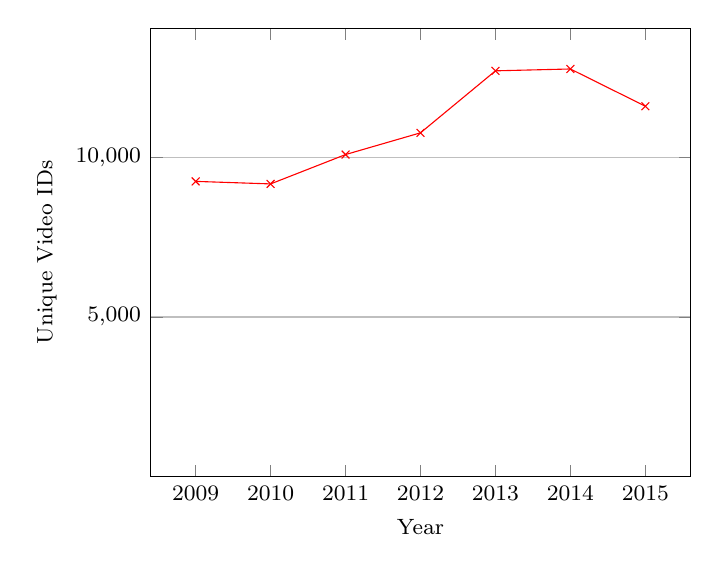
\begin{tikzpicture}
        \begin{axis}[
            ymin = 0,
            xlabel = Year,
            ylabel = Unique Video IDs,
            font = \footnotesize,
            xtick = {1, ..., 7},
            xticklabels = {2009, 2010, 2011, 2012, 2013, 2014, 2015},
            ytick = {5000, 10000},
            scaled y ticks = false,
            ymajorgrids = true
            ]
            \addplot[color=red, mark=x] coordinates {
                (1, 9248)
                (2, 9169)
                (3, 10089)
                (4, 10770)
                (5, 12712)
                (6, 12770)
                (7, 11603)
            };
       %     \addplot[color=blue, mark=*] coordinates {
       %         (1, 8793)
       %         (2, 9180)
       %         (3, 10038)
       %         (4, 8218)
       %         (5, 10205)
       %         (6, 11933)
       %         (7, 11603)
       %     };
        \end{axis}
    \end{tikzpicture}
    \caption{Unique video IDs for January, by year}
    \label{jan-ids-year}
\end{figure}



\begin{tikzpicture}
	\begin{axis}[
		xlabel=Month,
		ylabel=Unique Video IDs]
	\addplot[color=red,mark=x] coordinates {
		(1,11603)
        (2,11194)
        (3,12907)
        (4,11581)
        (5,11572)
        (6,11609)
        (7,11410)
        (8,12716)
        (9,120304)
        (10,319270)
    };
    \addplot[color=blue,mark=*] coordinates {
        (1,11603)
        (2,11402)
        (3,12905)
        (4,11581)
        (5,11527)
        (6,11640)
        (7,11206)
        (8,12709)
        (9,110822)
        (10,1280155)
    };
	\end{axis}
\end{tikzpicture}


\begin{tikzpicture}[y=.2cm, x=.7cm,font=\sffamily]
 	%axis
	\draw (0,0) -- coordinate (x axis mid) (10,0);
    \draw (0,0) -- coordinate (y axis mid) (0,30);
    %ticks
    \foreach \x in {0,...,10}
    \draw (\x,1pt) -- (\x,-3pt)
        node[anchor=north] {\x};
    \foreach \y in {0,5,...,30}
        \draw (1pt,\y) -- (-3pt,\y);
            node[anchor=east] {\y}; 
	%labels      
	\node[below=0.8cm] at (x axis mid) {Day};
	\node[rotate=90, above=0.8cm] at (y axis mid) {Unique video IDs};

	%plots
	\draw plot[mark=*, mark options={fill=white}] 
		file {video_ids_october.data};    
\end{tikzpicture}



\section{Future work}
%\lipsum[1-4]
\section{Future work}
Perhaps the most obvious issue to address in future work is the inconsistancy
of the YouTube API. Doing research on what causes inconsistent replies could
initially improve the effectivity of the developed tool, but perhaps more 
importantly it could be used to improve the YouTube API. 

Investigating why the API return rate drops dramatically at certain intervals
when looking back in time, and looking at what kind of videos that disappear
from the returned set, will give interesting knowledge about the YouTube API,
as well as perhaps give a final answer to whether the returned video set is
indeed biased.

There are many conceivable additions to the tool as it is now. Improving the
statistics view could improve the user experience and make it easier for the
user to make decisions about what to do next. A feature that allows the user to
export a database containing only a selected set of videos could drastically
reduce SQL query times during analysis, and we would recommend making some
feature like this if SQL querying becomes a major time and resource consumer.

There is a lot of room for performance improvements, especially when it comes to
concurrency. The tool was tested on a variety of platforms, and performed
reasonably well on most of them, but on certain configurations the API requests
were inexplicably horrendously slow. The cause of this might be a weird
combination of hardware, drivers, and TCP implementation in the OS kernel - 
we simply had no time to narrow down the possible causes. Adding support to run
multiple Celery jobs per task might have alleviated some of the performance
hangups.



\section{Conclusion}
This article presented the YouTube implementation of DASH compared to 
ISO/IEC 23009-1. It gave an overview of the YouTube Data API v3, outlined
the major limitations of it and also provided some guidelines on how to
bypass these limitations in order to obtain a good sample of YouTube
videos for further analyzes. The main decision criteria on implementing
the searching for videos were concurrency and maximization of the amount
of responded videos while minimizing the quota costs and requests needed
to achieve this. While creating the tool, there were 2305 open issues
associated to the YouTube API on the Google Data APIs issue tracking
platform ~\cite{conclusion:gdataissue} and some of them were related to
the behaviors we have experienced.


%\lipsum[1-4]

%\bibliography{bibliography}{}
%\bibliographystyle{plain}
\begin{thebibliography}{1}
	\bibitem{conclusion:gdataissue}
		Google Code server-side issues and feature requests for YouTube Data API v3
		https://code.google.com/p/gdata-issues/issues/list?q=label:API-YouTube
\end{thebibliography}


\end{document}
